\documentclass[11pt,a4paper,titlepage]{article}
\usepackage[utf8]{inputenc}
\usepackage[english]{babel}
\usepackage[T1]{fontenc}
\usepackage{amsmath}
\usepackage{amsfonts}
\usepackage{amssymb}
\usepackage{todonotes}
\usepackage{fullpage}

\title{INGI2141 Project 1\\-- Reliable Transfer Protocol --}
\author{Laurent Quentin (4834-11-00)\\Lacomblez Loïc (2756-11-00)}

\newcommand{\blank}{\vspace{11pt}}

\begin{document}
\maketitle

\section*{Introduction}
For this first project for the course \textsc{ingi}2141, we had to implement a reliable transfer protocol on top on \textsc{udp}. Two programs use this protocol : \texttt{sender} and \texttt{receiver}. The objective is to share a given file in a mono-directional fashion, that is to say with the sender only sending data packets containing the file and the receiver only sending acknowledgements packets. This report briefly presents the program architecture, then gives an overview of the sending and receiving routines. In the end, informations about the interoperability tests that we carried and a brief discussion about the program limitations are provided.

\section{Implementation}


\subsection{Protocol and Program organization}
The \texttt{sender} and the \texttt{receiver} programs both use a small library called \texttt{rtp.h}. In this file, we defined the packet structure of our protocol, as specified in the project statement. Figure \ref{fig:struct} describes this structure. With this header format, we can have a window size up to 31 and sequence numbers from 0 to 255.

\texttt{rtp.h} also contains the structure used to represent a single slot of the programs' sliding windows. This structure contains three fields : a \textbf{sequence number}, a \textbf{receive flag} that is set to true if the packet (resp. the acknowledgement) with this sequence number has been received, and a \textbf{time entry} that corresponds to the moment when the packet was sent, used to implement the resend timer.

Finally, \texttt{rtp.h} contains three common routines used by the program to instanciate a socket, as well as to compute and check the packets' \textsc{crc}. Our implementation uses the function \texttt{crc32} defined in \texttt{zlib.h}.

\begin{figure}[!ht]
	\centering
	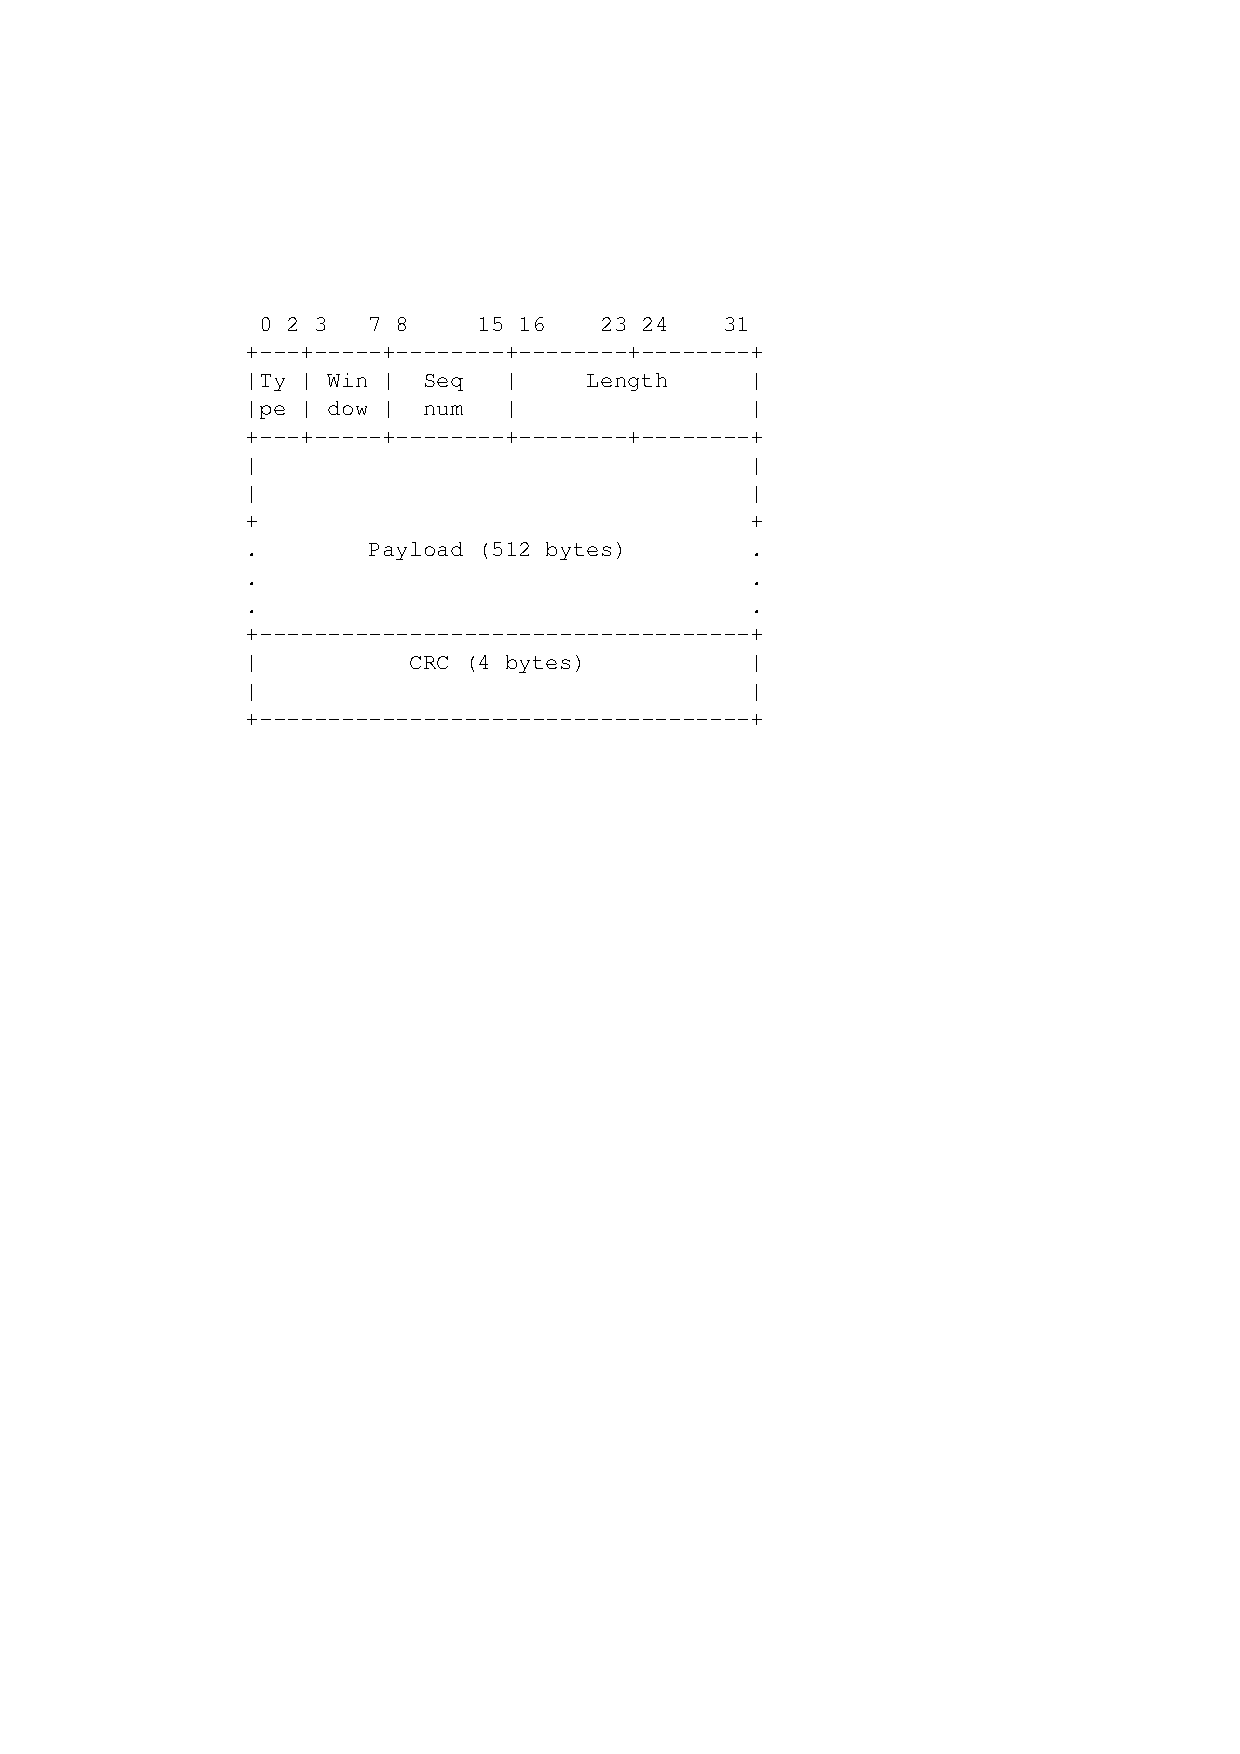
\includegraphics[width=.5\textwidth]{figure/packet_header.pdf}
	\caption{\label{fig:struct} Protocol Packet Structure}
\end{figure}

\subsection{Sender Program}

The main function delegates the majority of the work to the \texttt{selectiveRepeat} function that implements the whole sending algorithm, from the file reading to the acknowledgements processing. 

\subsubsection{Algorithm main steps}
The sending routine consists in a while loop that stops when all the packets forming the file have been sent and acknowledged by the receiver. At each iteration, the sender executes the following steps in sequence :
\begin{enumerate}
\item Fill in the sending buffer until its maximal capacity is reached. Of course, only the already acknowledged packets are overwritten.
%
\item For each new packet that has been added at this iteration, directly send them to the receiver.
%
\item Check if an acknowledgement has been received. If so, check the window size specified in it to adapt the window and sending buffer if needed. 
%
\item Mark the acknowledged packets from the sending buffer as ‘‘received’’. They are then ready to be removed and overwritten by new packets.
%
\item Check if a timer associated with a packet has expired. If it has, then the packet is sent again.
\end{enumerate}
Thus, the tasks of sending and receiving acks are done sequentially. This simplifies the code, but increases the delay between the receiving of an ack and the sending of new packets. However, this delay remains relatively short, and a multithreaded implementation wouldn't give substantial performance improvements. 

\subsubsection{Window representation}
We represent the window as an array of \texttt{window\_slot} structures. The conceptual \emph{sliding movement} of the window over consecutive sequence numbers is replaced by a fixed array where the sequence numbers are incremented in a rotating fashion.
Figure \ref{fig:sliding_win} illlustrates this concept by comparing the usual sliding window representation with the one we used. On this figure, we slide the window by two sequence numbers.
\begin{figure}[!ht]
	\centering
	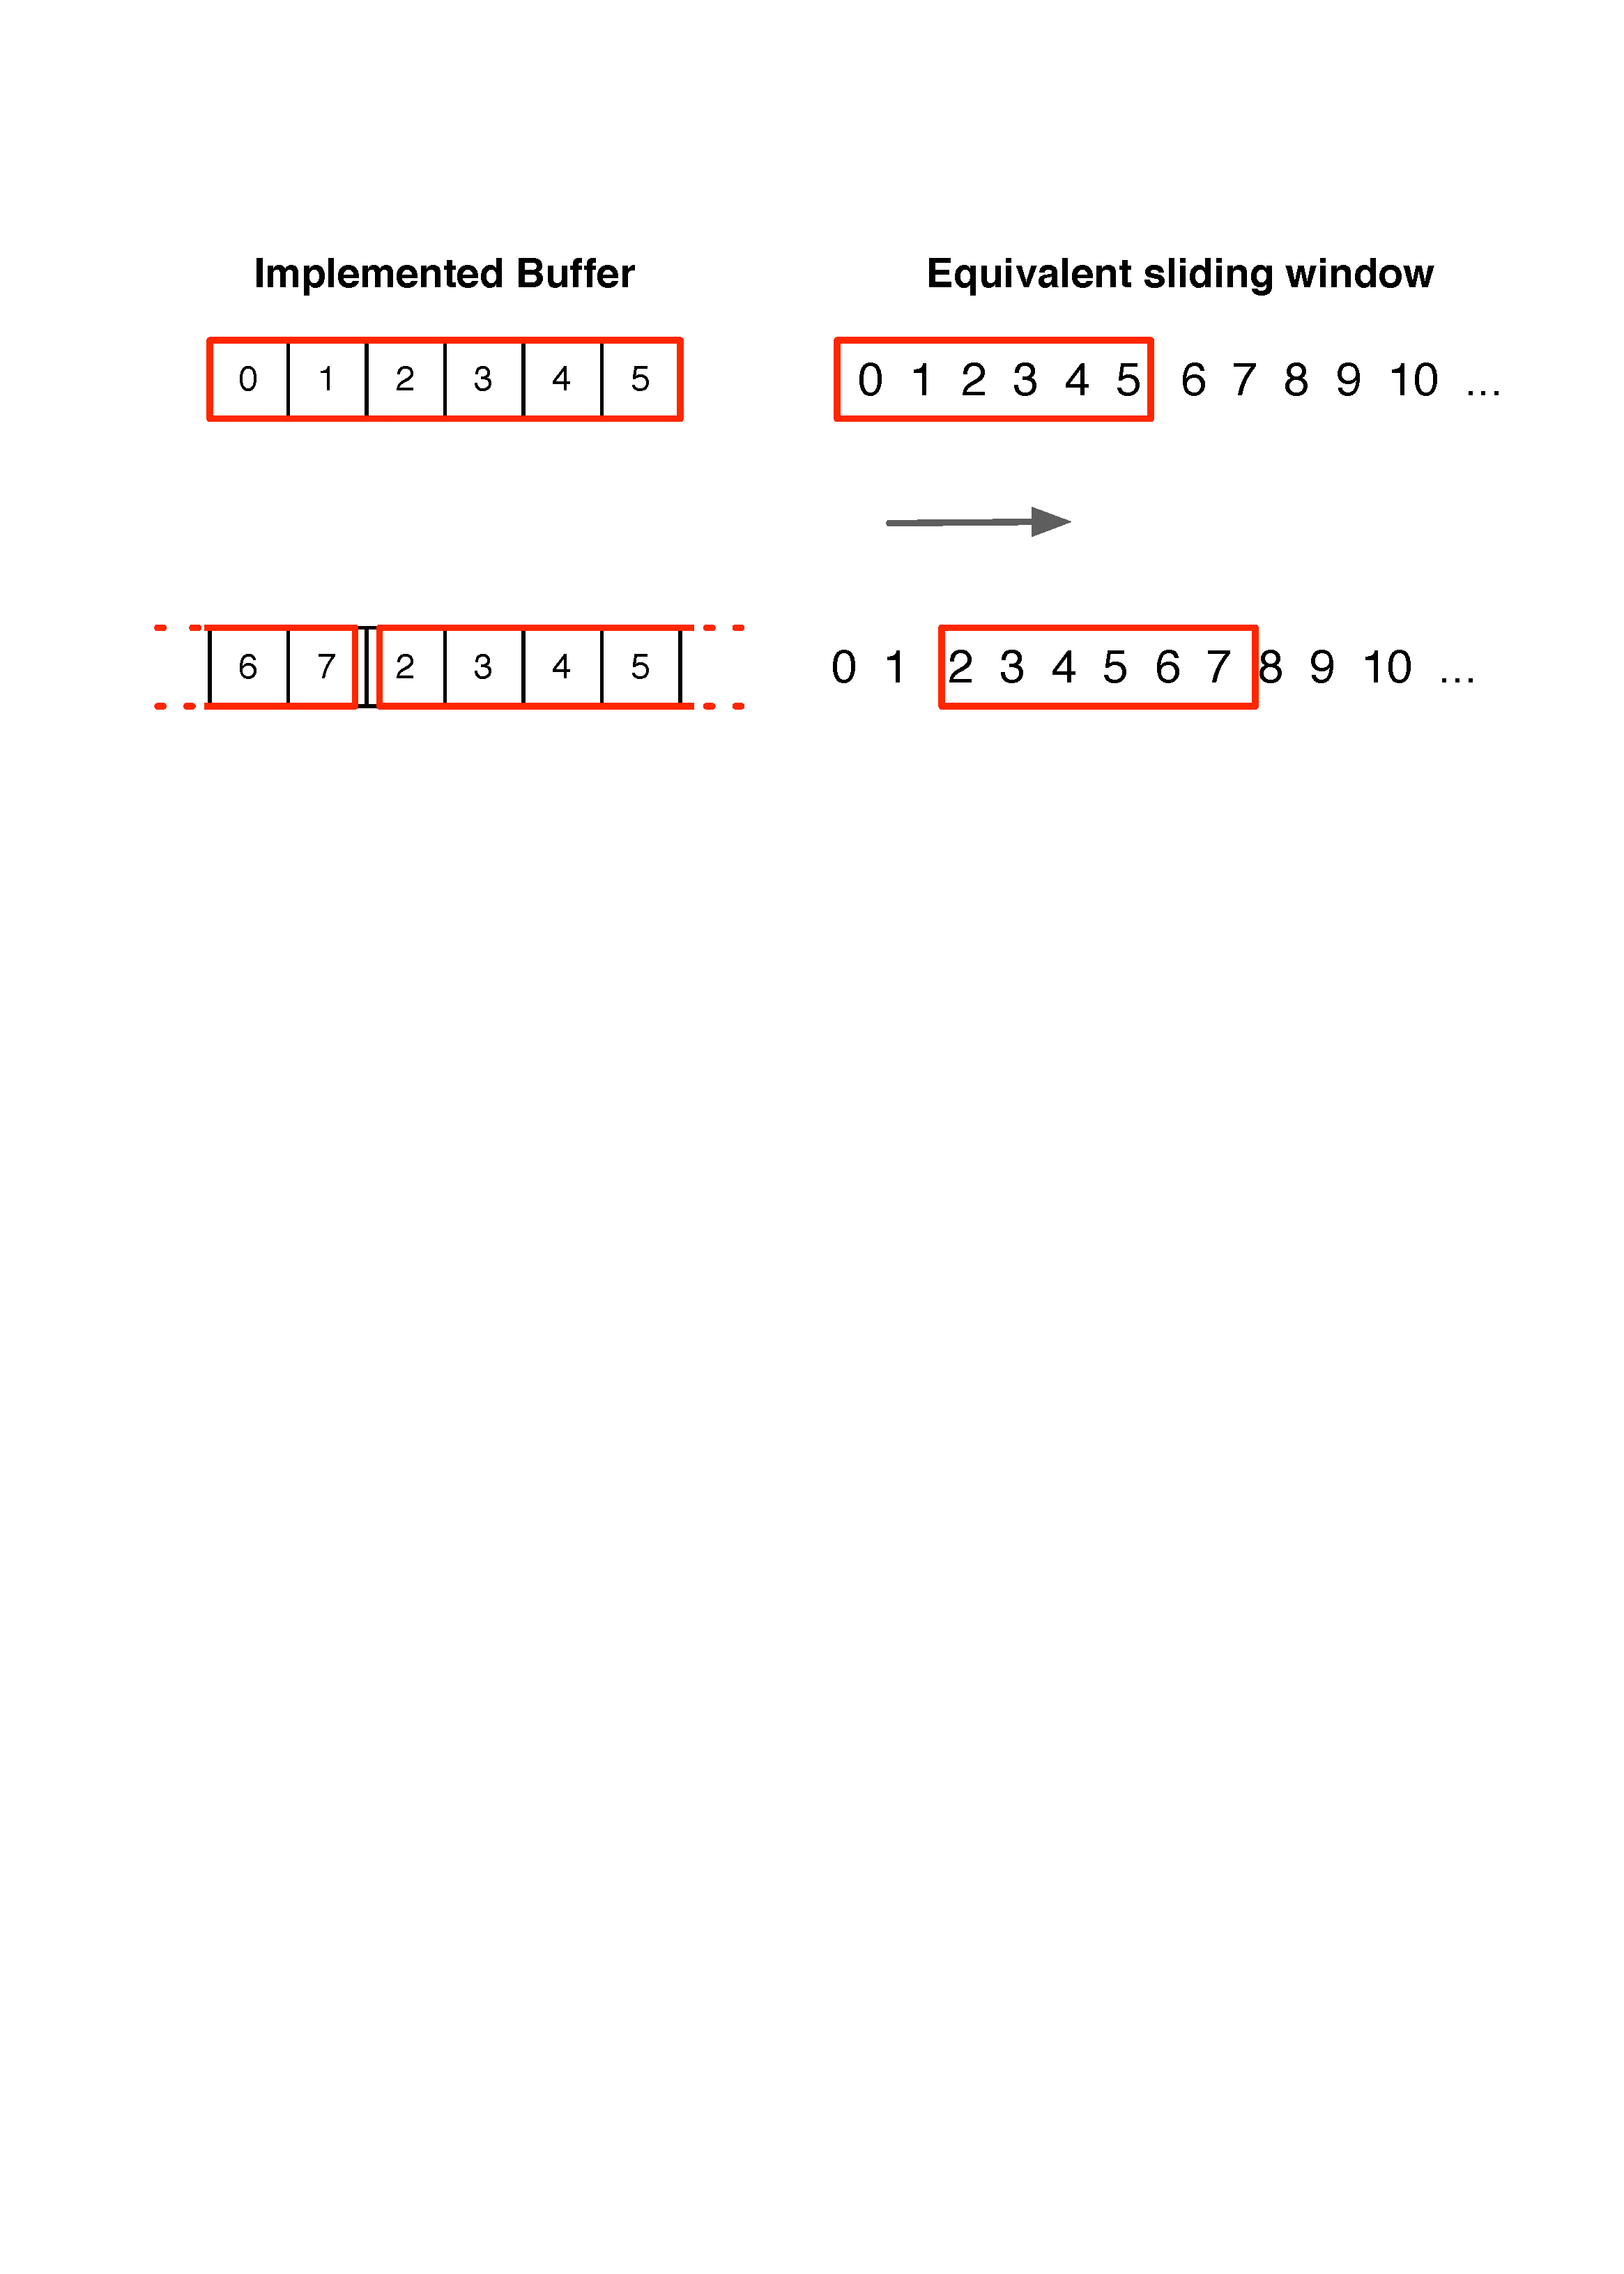
\includegraphics[width=.7\textwidth]{figure/sliding_win.pdf}
	\caption{\label{fig:sliding_win} Illustration of the sliding window buffer}
\end{figure}


\subsubsection{Management of the sending buffer}

We use 4 variables to maintain the state of the window. First, \texttt{seq} and \texttt{unack} are relative to the sequence numbers of packets. \texttt{seq} is the sequence number of the next packet to send, while \texttt{unack} is the sequence number of the last acknowledgement received. The indices of the corresponding packets in the sending buffer would be \texttt{bufferPos} and \texttt{bufferPos-bufferFill}, where \texttt{bufferFill} is the number of packets currently in the buffer, all of which have already been sent.
Figure \ref{fig:sending_win} shows the position of those different variables on the window. The gray part is the actual array implemented in our program, the white part is the other sequence numbers the window is sliding on, as represented on the right side of figure \ref{fig:sliding_win}. The variables on the top represent the sequence numbers stored in the slots, while the bottom shows the indices in the array. Of course, modulo's are to be applied on those indices, but we conceptually neglect them in the illustration.
\begin{figure}[!ht]
	\centering
	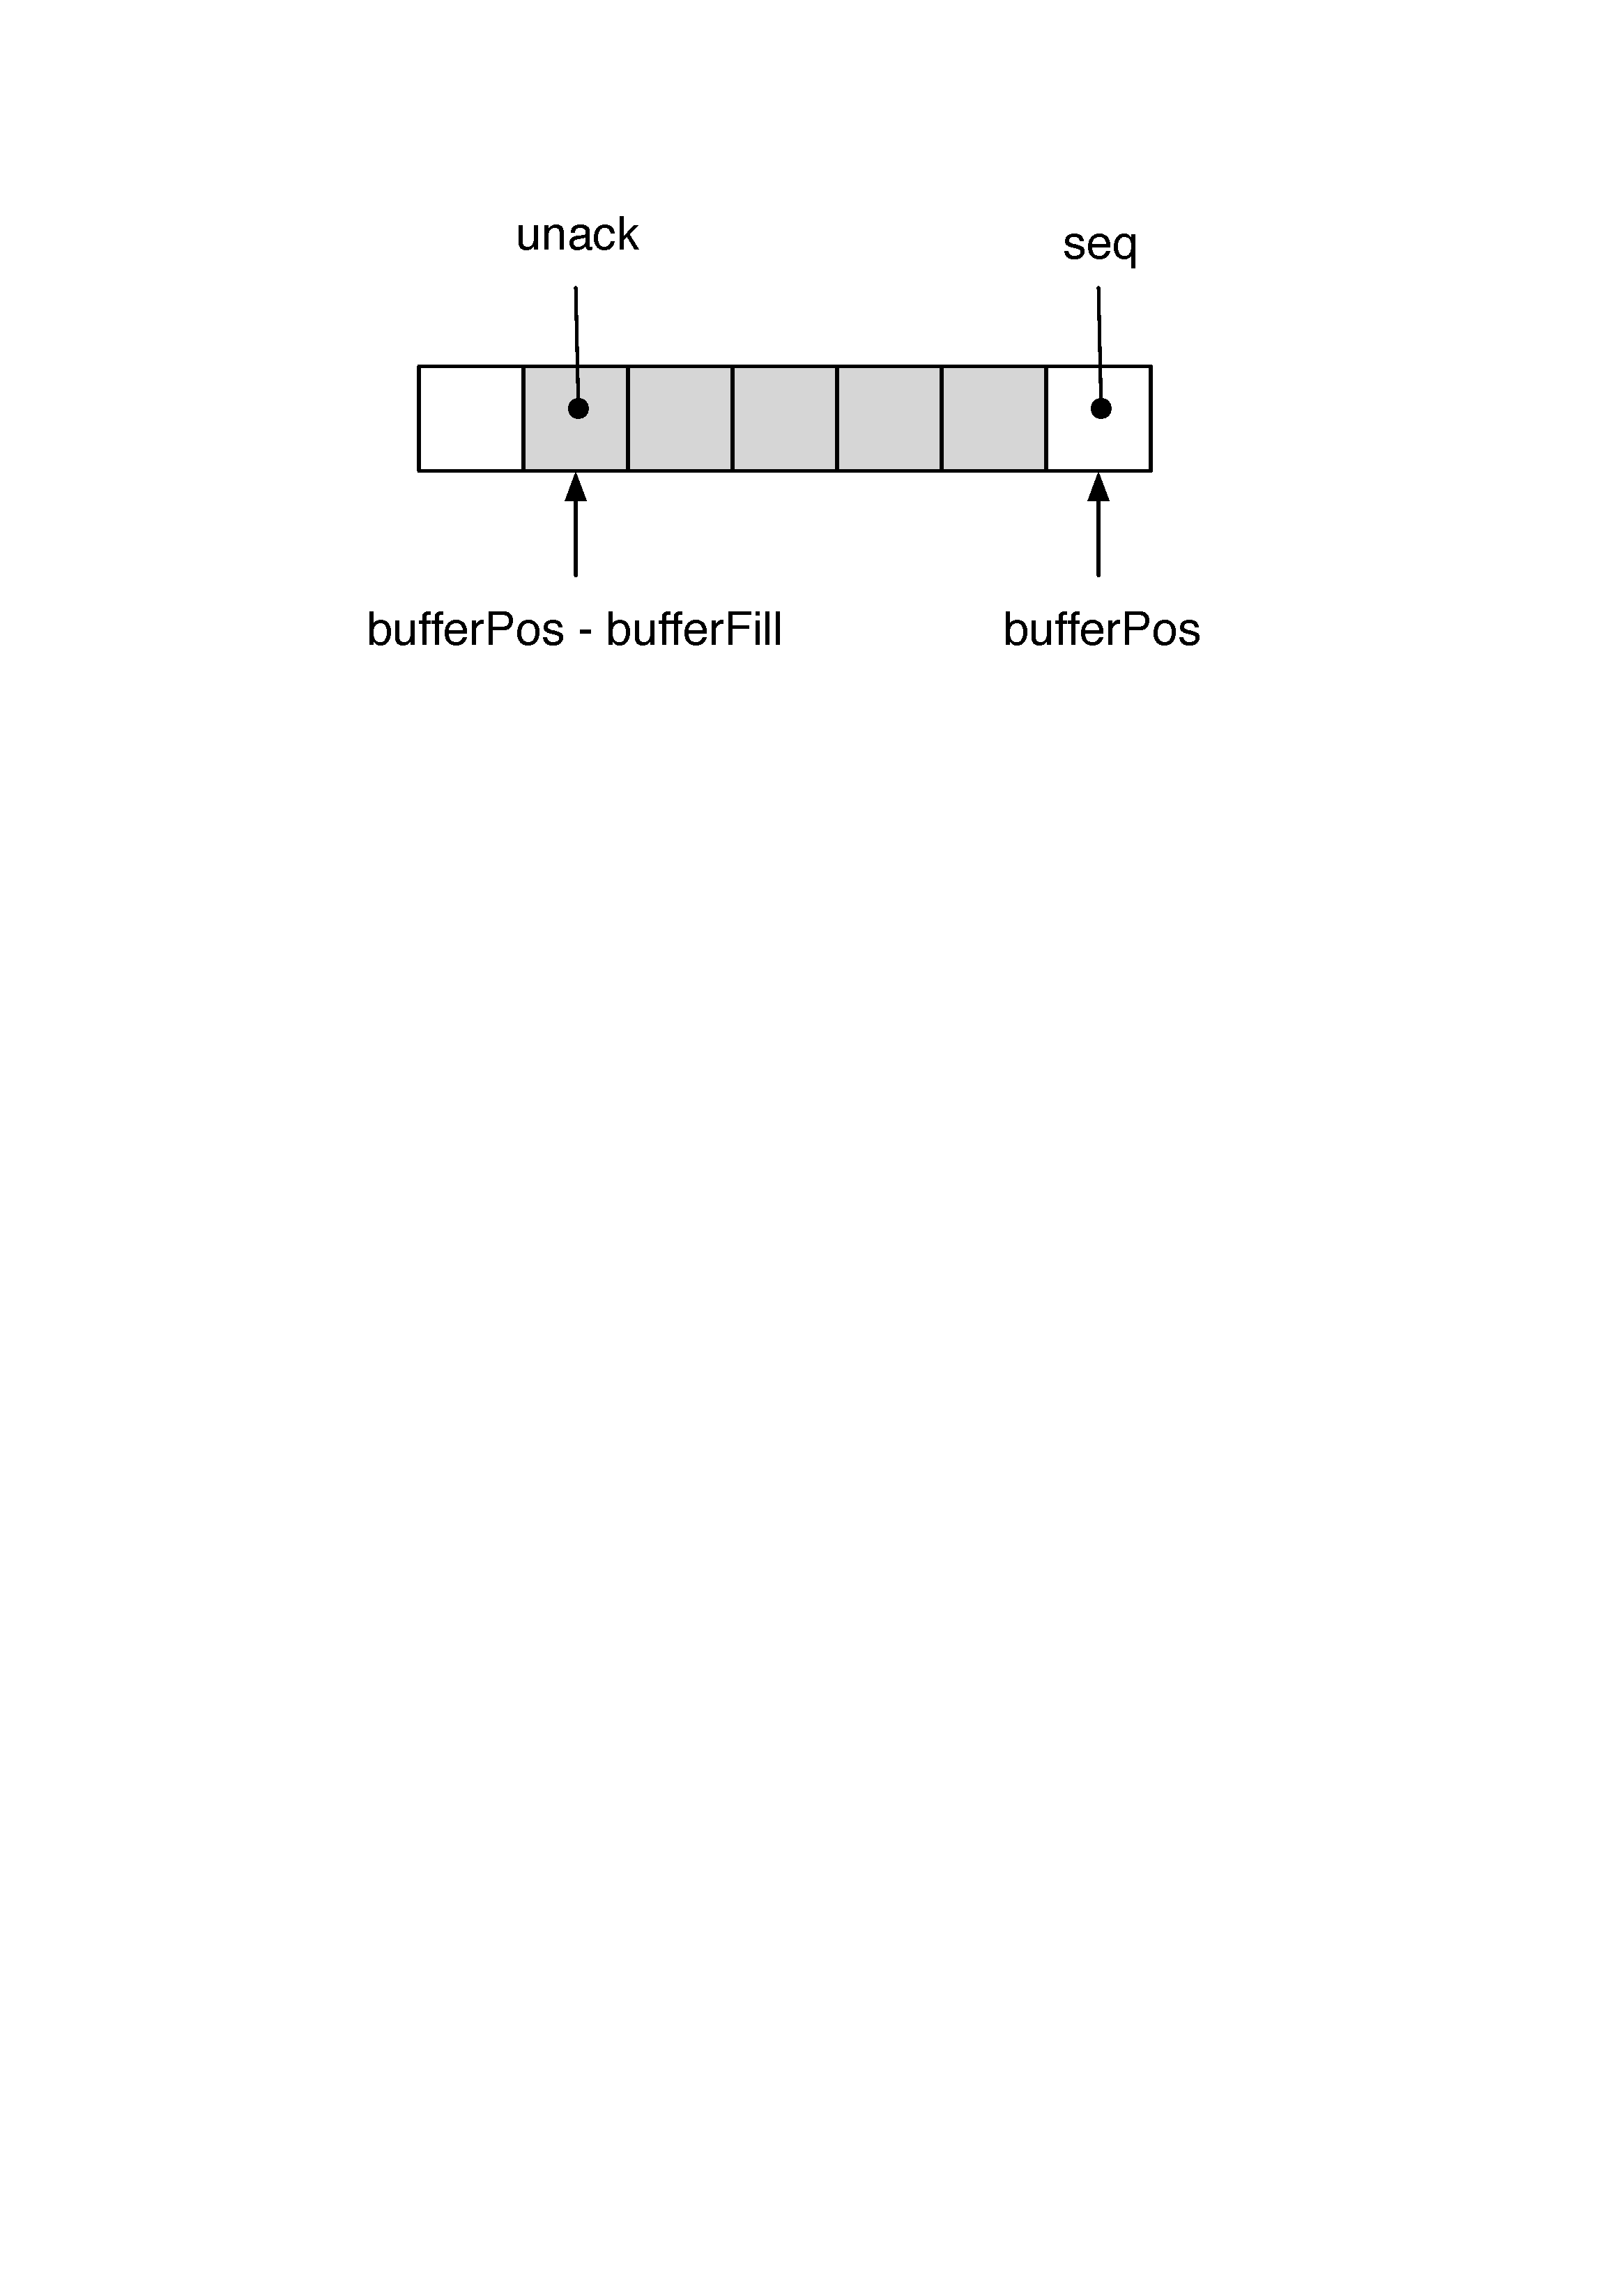
\includegraphics[width=.4\textwidth]{figure/sending_buf.pdf}
	\caption{\label{fig:sending_win} Illustration of the sender's window}
\end{figure}


\subsection{Receiver Program}
The way the receiving window and buffer are modeled is pretty much the same as for the sender's ones. However, the different pointers concerning the receiving buffer have a different meaning here. Figure \ref{fig:recv_win} shows the variables used, in the same fashion as for the sender.
\begin{figure}[!ht]
	\centering
	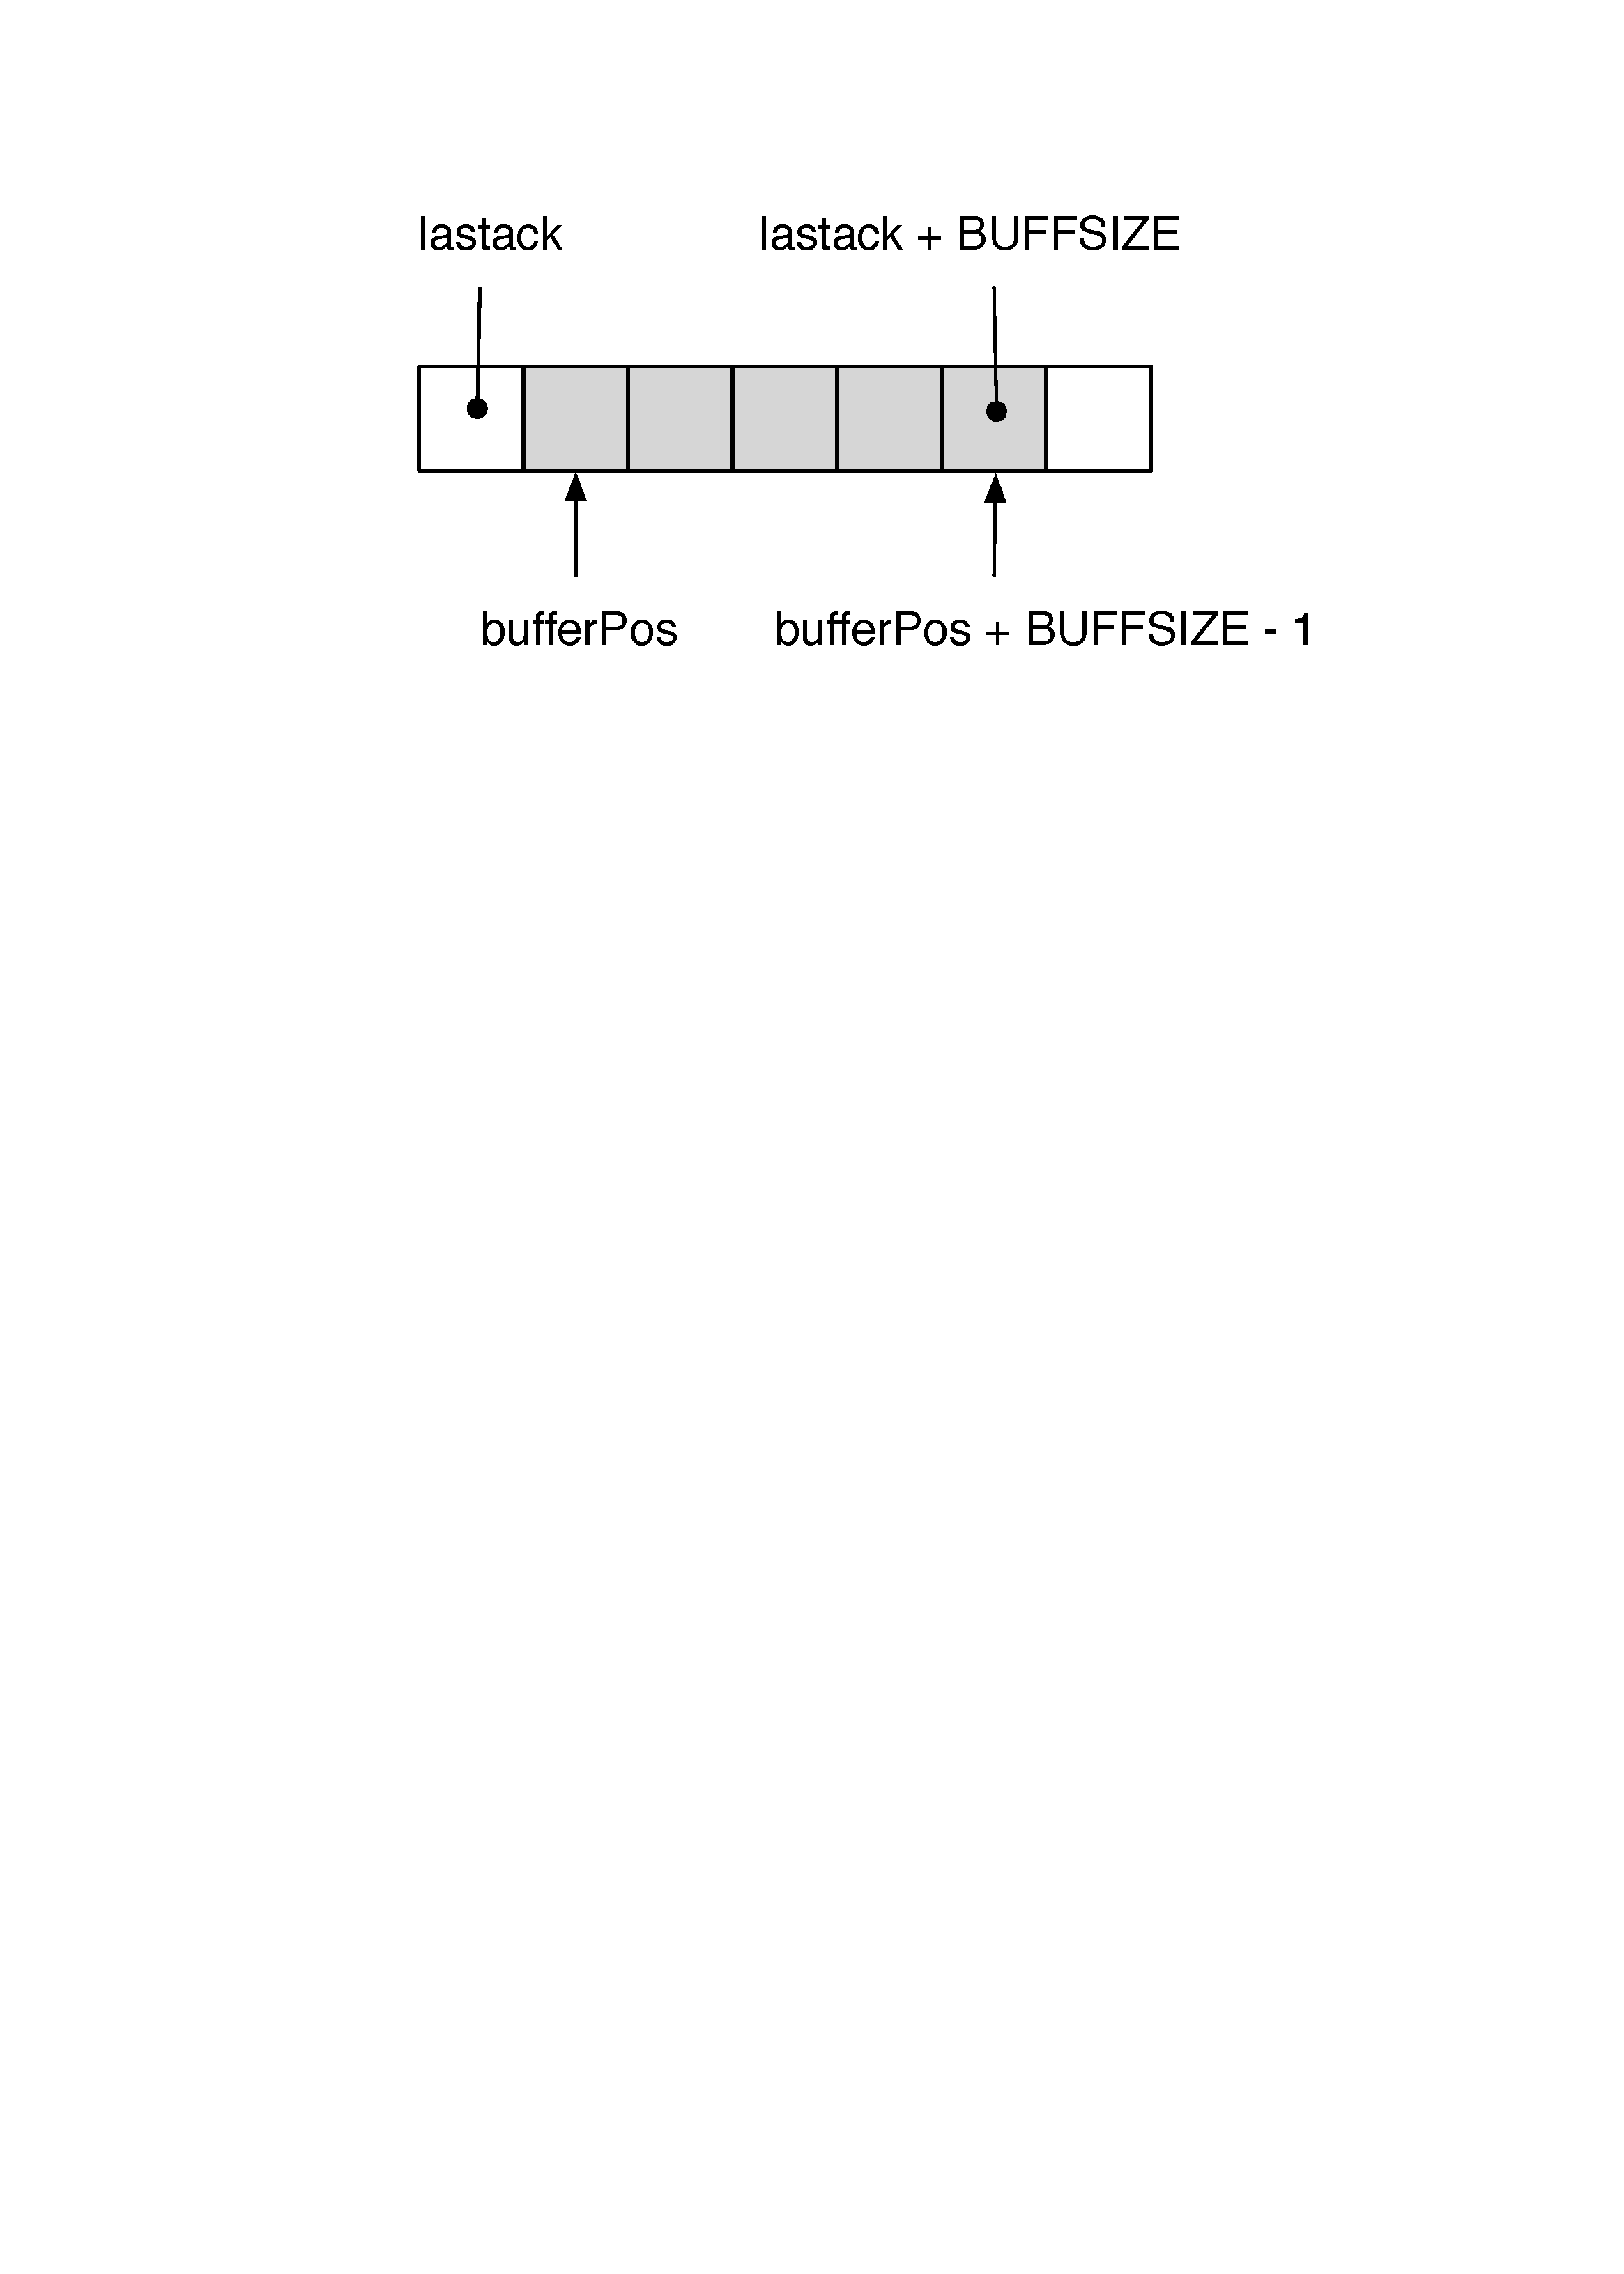
\includegraphics[width=.4\textwidth]{figure/receiving_win.pdf}
	\caption{\label{fig:recv_win} Illustration of the sender's window}
\end{figure}

\subsubsection{Algorithm main steps}
The receiver is also implemented by a \texttt{while} loop, that terminates once the whole file has been received. We determine that the file has been entirely received if a packet with a \texttt{length} field smaller than the usual 512 bytes payload size has been received, and when the variable \texttt{lastack} is equal to the sequence number of this last packet.\\
At each iteration, the following steps are executed in sequence :
\begin{enumerate}
\item Wait until a packet is received. If it is corrupted (ie, an error is found when computing the \texttt{crc}) drop it and loop again. Else, follow the next steps.
%
\item If the received packet's sequence number is out of the receiving window, discard it and loop again. Else, compute the index where to insert it in the receive buffer and follow the next steps.
%
\item Place the packet in the receiving buffer at the index computed in the previous step.
%
\item Iterate from the packet that has sequence number \texttt{lastack + 1} and write in the destination file all the consecutive packets that have been received. Update the sequence numbers in the receiving window accordingly to be ready to receive next packets.
%
\item Update \texttt{lastack} and send an acknowledgement with sequence number \texttt{lastack + 1}.
\end{enumerate}

\section{Interoperability tests}
We have carried out two interoperability tests, always testing the functionality in both sending and receiving direction. For this purpose, Wireshark has been very helpful to determine which program was faulty. Surprisingly enough, we encountered few issues. The principal was when using another group's sender with our receiver.
\blank

We have assumed that the sequence number must continuously increase from 0 to 255, and then be reset to 0 and increase again. This is, in our sense, logical because not using all the 8 bits dedicated to it would be a waste of space, and it's also better because we could use much larger windows without having to rethink the way sequence numbers are managed. However, the other group implementation was sending sequence numbers ranging from 0 to 30. Since our receiver isn't expecting those sequence number, the transmission blocked.


\section{Known Limitations}
Here is an overview of our implementation limitations we've been thinking about :
\begin{enumerate}
\item Because the payload of the acknowledgement packets must be zero, we can't include the content of the receiving window in it. So, when an out-of-sequence packet is received, the whole sequence of packets from \texttt{lastack} to the current packet will be sent again if a timeout occurs. 
%
\item The end of the transmission is a bit tricky. Because our protocol isn't connection-oriented, we can only make a hard disconnect, and the last acknowledgement packet could be lost, causing the sender to send it again indefinitely. In order to handle this, we decided to keep the receiver listenning a short time after it has received all the packets, so that it can send again an acknowledgement to the sender. Of course, there are no strict guarantee that this will work.
%
\item The timer delay for each packet we send is statically defined. A better approach would be to set it according to the transmission delay. 
%
\item Our program doesn't handle receiving window size variation. The transmission will still be on if we change window size, but the last packets that are now out of the window would be systematically dropped. 

\end{enumerate}
\end{document}
